\section{Results and Discussion} \label{sec:results_discussion}
This section presents the results of the security analysis and performance measurements, followed by a discussion of the findings.

\subsection{Security Analysis Results}
The effectiveness of VxLang virtualization was evaluated through static and dynamic analysis attempts to understand and bypass the authentication logic in the case study applications.

\subsubsection{Static Analysis (Ghidra)}
\begin{itemize}
	\item \textbf{Non-Virtualized Binaries:} Analysis of non-virtualized binaries was generally straightforward. Relevant strings and control flow for authentication logic were typically identifiable. For instance, in the non-virtualized \texttt{app\_qt.exe}, while a specific recent Ghidra analysis reported an unusually low count of 0 instructions and only 2 functions (possibly an analytical anomaly for that run, with 1279 defined data entries and 226 symbols, compiler identified as `clangwindows`, size 125,864 bytes), the typical expectation for such binaries is observable logic. Standard comparison instructions and conditional jumps were readily found in other non-virtualized samples (see Appendix Listings \ref{lst:asm_static_nonvirt_full}, \ref{lst:asm_static_cloud_full}), making static patching feasible.

	\item \textbf{Virtualized Binaries:} Static analysis proved significantly more challenging for binaries processed by VxLang.
	      \begin{itemize}
		      \item \textit{Instruction and Function Obscuration:} For the virtualized \texttt{app\_qt\_vm.vxm.exe}, Ghidra consistently failed to recognize standard x86-64 instructions, reporting 0 instructions and 0 functions. This starkly contrasts even with the anomalous low detection in the original, indicating a fundamental transformation of the code into a format uninterpretable by standard disassembly.
		      \item \textit{Data and Symbol Reduction:} Critical data was obscured. The count of defined data entries in \texttt{app\_qt\_vm.vxm.exe} dropped to 174 from 1279 in the original, and symbols decreased from 226 to 33. This impedes the identification of code sections via string or symbol searches. The compiler was also reported as `unknown`.
		      \item \textit{File Size Increase:} The file size for \texttt{app\_qt\_vm.vxm.exe} increased substantially to 2,008,495 bytes from 125,864 bytes (approximately 15.95 times larger), indicative of the embedded VM and bytecode.
		      \item \textit{Control Flow Obscurity:} The clear structure of conditional checks and jumps seen in original, easily analyzable code was replaced by opaque sequences, rendering static identification and patching of the core authentication logic nearly impossible. The control flow graph became fragmented and uninformative.
	      \end{itemize}
Static analysis proved significantly more challenging for binaries processed by VxLang. The observed failure of Ghidra to recognize standard x86-64 instructions (reporting 0 instructions and functions for \texttt{app\_qt\_vm.vxm.exe}) and the drastic reduction in defined data and symbols are direct consequences of code virtualization. As outlined in Section \ref{sec:related_work}, static disassemblers are designed for native ISAs \cite{Sikorski2012, Eilam2011}. VxLang transforms the original code into a custom bytecode format, rendering it uninterpretable by Ghidra, which attempts to map these bytes to an x86-64 ISA for which they are not valid \cite{Ko2007}. The substantial file size increase further indicates the embedding of the VM runtime and the transformed bytecode.
	      Static bypass attempts on virtualized binaries were unsuccessful due to the inability to locate and comprehend the relevant control flow logic. Consequently, static identification and patching of the core authentication logic became practically impossible. The figures referenced (e.g., Fig. \ref{fig:ghidra_summary_qt_journal} and Fig. \ref{fig:ghidra_summary_qt_vm_journal} in the main thesis document) visually demonstrate these differences.
\end{itemize}


% --- Ghidra Summary Figures (Journal) ---
\begin{figure}[!t]
	\centering
	\includegraphics[width=0.9\linewidth]{../assets/pics/app_qt_summary_result.jpeg}
	\caption{Ghidra Analysis Summary for \texttt{app\_qt.exe} (Non-Virtualized).}
	\label{fig:ghidra_summary_qt_journal}
\end{figure}

\begin{figure}[!t]
	\centering
	\includegraphics[width=0.9\linewidth]{../assets/pics/app_qt_vm_summary_result.jpeg}
	\caption{Ghidra Analysis Summary for \texttt{app\_qt\_vm.exe} (Virtualized, showing data for app\_qt\_vxm.exe structure).}
	\label{fig:ghidra_summary_qt_vm_journal}
\end{figure}

\subsubsection{Dynamic Analysis (x64dbg)}
\begin{itemize}
    \item \textbf{Non-Virtualized Binaries:} Dynamic analysis of non-virtualized binaries using x64dbg was generally straightforward. Setting breakpoints based on string references or near conditional jumps identified during static analysis proved effective. Stepping through the code clearly revealed the comparison logic and the execution of conditional jumps. Runtime patching of these jump instructions directly in x64dbg successfully bypassed authentication mechanisms, corroborating static analysis findings. (See example context in thesis Appendix Listing \ref{lst:asm_dynamic_nonvirt_full}).

    \item \textbf{Virtualized Binaries:} Dynamic analysis of VxLang-virtualized binaries (e.g., \texttt{app\_qt\_vm.vxm.exe}) presented a more nuanced challenge.
    \begin{itemize}
        \item \textit{Visibility of Native VM Instructions:} Once the virtualized Qt application was fully loaded and its GUI rendered, x64dbg \textbf{was able to display valid native x86-64 instructions} being executed. Snippets such as \texttt{sub rsp,48}, \texttt{mov}, \texttt{cmp}, and \texttt{jne} (referring to addresses within the virtualized module, e.g., \texttt{app\_qt\_vm.vxm.7FF64A6A105D}) were observable. These instructions are understood to be part of the VxLang Virtual Machine (VM) interpreter itself, which is native code responsible for executing the virtualized application's bytecode. Initial, less clear instructions (e.g., repetitive \texttt{add byte ptr ds:[rax],al}) seen before the application fully loaded likely correspond to VxLang's loader or initialization routines. 

        \item \textit{Persistent Obscurity of Critical Data and Application Logic:} Despite the visibility of the VM's native instructions, the core challenges in dynamic analysis persisted:
            \begin{itemize}
                \item \textbf{String Obfuscation:} Critical strings that were explicitly virtualized within the source code (e.g., "Authentication Failed", "Authentication Success") \textbf{could not be located} using standard string reference searches or memory scanning techniques within x64dbg during runtime. However, non-virtualized strings (e.g., static UI text not covered by VxLang macros) were generally still discoverable. This highlights VxLang's effectiveness in protecting targeted string literals.
                \item \textbf{Abstraction of Application Logic:} The primary difficulty lay in the fact that the application's original logic (e.g., credential comparison, decision-making for authentication) was transformed into an internal bytecode representation executed by the VxLang VM. Therefore, x64dbg showed the execution of the VM's interpreter, not the direct native execution of the application's original high-level logic. Understanding how the VM's operations mapped back to the original application's semantics remained a significant hurdle.
            \end{itemize}

        \item \textit{Ineffectiveness of Simple Runtime Patching:} Consequently, attempts to bypass authentication by patching simple conditional jumps at runtime—a successful technique for non-virtualized versions—were \textbf{rendered ineffective}. The critical decision-making points of the application logic were no longer exposed as easily identifiable native instructions but were embedded within the VM's execution flow.
    \end{itemize}
    These dynamic analysis findings align with the principles of VM-based obfuscation \cite{Sikorski2012, Ore06}. While the debugger can step through the native code of the VM interpreter, the actual application logic is abstracted away into a custom bytecode, making direct analysis and manipulation of the original program flow exceptionally difficult without a deep understanding of the specific VM's architecture and its bytecode-to-native instruction mappings \cite{Sal18}.
\end{itemize}

These results strongly indicate that VxLang's code virtualization effectively hinders both static and dynamic reverse engineering attempts using standard tools and techniques.

\subsubsection{Analysis of Lilith RAT}

After careful and iterative placement of VxLang macros, functional testing confirmed that the virtualized Lilith client (\texttt{Lilith\_Client\_vm.vxm.exe}) remained fully operational. Initial, broader applications of virtualization macros to large code blocks within Lilith, especially around complex control flow constructs (e.g., switch-cases for packet processing) or I/O operations (e.g., \texttt{SendString} calls), led to functional issues such as application crashes when specific commands like \texttt{remoteControl cmd} were triggered. Stable operation, as demonstrated in a two-machine local network setup (client IP: \texttt{192.168.1.15}, server IP: \texttt{192.168.1.235}, port \texttt{1337}), was achieved by refining macro placement to target more specific, self-contained critical functions. The virtualized client successfully connected to the unmodified Lilith server, allowed remote command prompt access, and facilitated remote file reading (\texttt{password.txt} containing \texttt{"THIS IS A SECRET"}). This confirmed that, with precise application, VxLang's virtualization can preserve core RAT functionalities (network communication, command execution, file system interaction) despite significant code transformation. This highlights the necessity of meticulous macro placement and thorough functional validation when applying such obfuscation to multifaceted software.

This indicates VxLang's virtualization can be applied to complex software, potentially including those with malicious characteristics, without necessarily breaking its intended functionality, while, as shown next, impacting its detectability.

\subsection{Performance and Size Overhead Results}

\subsubsection{Execution Time Overhead}
The performance impact was measured using QuickSort and AES benchmarks.

\begin{itemize}
	\item \textbf{QuickSort:} As shown in Table \ref{tab:quick_sort_performance_journal} and Fig. \ref{fig:quick_sort_performance_journal}, virtualization introduced substantial execution time overhead. The overhead increased with data size, ranging from approximately 27,300\% for 100 elements (0.01 ms to 2.74 ms) to about 15,150\% for 1,000,000 elements (218.32 ms to 33,292.91 ms). This indicates a significant constant overhead plus a scaling factor imposed by the VM's interpretation loop for the recursive sorting function.
	      \begin{table}[!t]
		      \centering
		      \caption{Quick Sort Execution Time Results (ms)}
		      \label{tab:quick_sort_performance_journal}
		      \resizebox{\columnwidth}{!}{%
			      \begin{tabular}{@{}lrrrr@{}}
				      \toprule
				      \multirow{2}{*}{\textbf{Array Size}} & \multicolumn{2}{c}{\textbf{Non-Virtualized}} & \multicolumn{2}{c}{\textbf{Virtualized}}                                        \\
				      \cmidrule(lr){2-3} \cmidrule(lr){4-5}
				                                           & \textbf{Avg Time}                            & \textbf{Std Dev}                         & \textbf{Avg Time} & \textbf{Std Dev} \\
				      \midrule
				      100                                  & 0.01                                         & 0.00                                     & 2.74              & 0.38             \\
				      1,000                                & 0.08                                         & 0.00                                     & 27.35             & 1.25             \\
				      5,000                                & 0.54                                         & 0.05                                     & 144.44            & 8.25             \\
				      10,000                               & 1.24                                         & 0.08                                     & 295.77            & 13.68            \\
				      50,000                               & 6.98                                         & 0.51                                     & 1,556.15          & 122.81           \\
				      100,000                              & 15.12                                        & 1.26                                     & 3,080.30          & 303.02           \\
				      500,000                              & 104.44                                       & 7.30                                     & 14,298.92         & 374.98           \\
				      1,000,000                            & 218.32                                       & 8.10                                     & 33,292.91         & 4,342.93         \\
				      \bottomrule
			      \end{tabular}
		      } % End resizebox
	      \end{table}

	      \begin{figure}[!t]
		      \centering
		      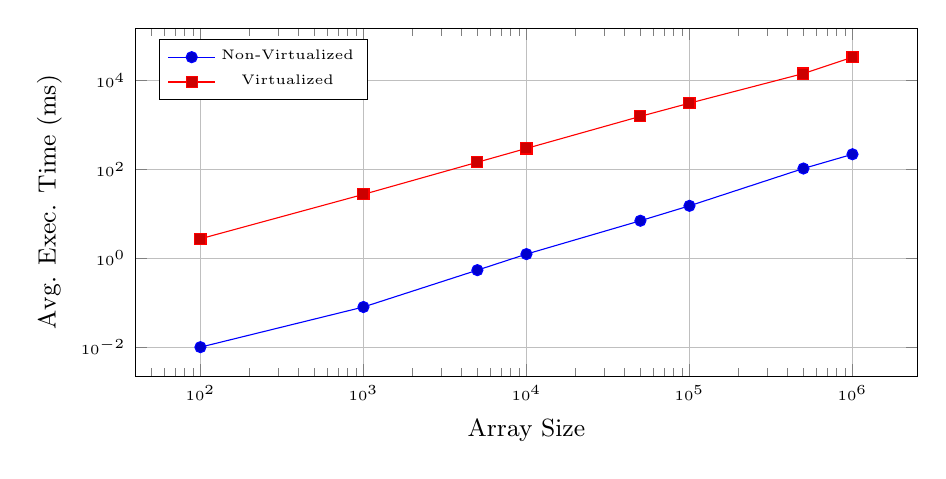
\begin{tikzpicture}
			      \begin{axis}[
					      width=0.95\columnwidth,
					      height=6cm,
					      xlabel={Array Size},
					      ylabel={Avg. Exec. Time (ms)},
					      xmode=log,
					      log basis x={10},
					      ymode=log,
					      log basis y={10},
					      legend pos=north west,
					      grid=major,
					      tick label style={font=\tiny},
					      label style={font=\small},
					      legend style={font=\tiny}
				      ]
				      \addplot coordinates {
						      (100, 0.01)
						      (1000, 0.08)
						      (5000, 0.54)
						      (10000, 1.24)
						      (50000, 6.98)
						      (100000, 15.12)
						      (500000, 104.44)
						      (1000000, 218.32)
					      };
				      \addlegendentry{Non-Virtualized};

				      \addplot coordinates {
						      (100, 2.74)
						      (1000, 27.35)
						      (5000, 144.44)
						      (10000, 295.77)
						      (50000, 1556.15)
						      (100000, 3080.30)
						      (500000, 14298.92)
						      (1000000, 33292.91)
					      };
				      \addlegendentry{Virtualized};
			      \end{axis}
		      \end{tikzpicture}
		      \caption{Quick Sort Execution Time Comparison (Log-Log Scale).}
		      \label{fig:quick_sort_performance_journal}
	      \end{figure}


	\item \textbf{AES Encryption:} Table \ref{tab:aes_performance_journal} shows that the total time for encrypting 976MB of data increased by approximately 396.7\% (1878.52 ms to 9330.73 ms), and decryption time increased by about 562.9\% (1304.75 ms to 8649.74 ms). Consequently, the combined throughput dropped dramatically from 634.16 MB/s to 108.78 MB/s (an 82.8\% reduction). This confirms a significant overhead for cryptographic operations.
	      \begin{table}[!t]
		      \centering
		      \caption{AES-256-CBC Performance Results (976MB Data)}
		      \label{tab:aes_performance_journal}
		      \resizebox{\columnwidth}{!}{%
			      \begin{tabular}{@{}lrr@{}}
				      \toprule
				      \textbf{Metric}              & \textbf{Non-Virtualized} & \textbf{Virtualized} \\
				      \midrule
				      Total Encryption Time (ms)   & 1,878.52                 & 9,330.73             \\
				      Total Decryption Time (ms)   & 1,304.75                 & 8,649.74             \\
				      Avg. Encrypt Time/Block (ms) & 0.00188                  & 0.00933              \\
				      Avg. Decrypt Time/Block (ms) & 0.00130                  & 0.00865              \\
				      Encrypt Throughput (MB/s)    & 519.86                   & 104.66               \\
				      Decrypt Throughput (MB/s)    & 748.46                   & 112.90               \\
				      Combined Throughput (MB/s)   & 634.16                   & 108.78               \\
				      \bottomrule
			      \end{tabular}
		      } % End resizebox
	      \end{table}

\end{itemize}

\subsubsection{File Size Overhead}
Table \ref{tab:file_size_journal} shows a consistent increase in executable file size after virtualization. For smaller console/benchmark programs (\texttt{quick\_sort}, \texttt{encryption}, \texttt{console}, \texttt{Lilith\_Client}), the size increased by over 15-18 times (from ~80-110 KB to ~1.5-1.6 MB). For larger GUI applications (\texttt{app\_imgui} from 1,675 KB to 2,330 KB; \texttt{app\_qt} from 122 KB to 1,578 KB) and the benchmark with embedded data (\texttt{size} from 97,771 KB to 112,324 KB), the relative increase was smaller but still significant. This overhead is primarily attributed to the inclusion of the VxLang VM runtime and the bytecode representation of the original code.
\begin{table}[H]
	\centering
	\caption{Executable File Size Comparison (KB)}
	\label{tab:file_size_journal}
	\resizebox{\columnwidth}{!}{
		\begin{tabular}{@{}lrr@{}}
			\toprule
			\textbf{Program}  & \textbf{Non-Virtualized (KB)} & \textbf{Virtualized (KB)} \\
			\midrule
			quick\_sort       & 98                            & 1,537                     \\
			encryption        & 110                           & 1,507                     \\
			size              & 97,771                        & 112,324                   \\
			console           & 92                            & 1,577                     \\
			console\_cloud    & 281                           & 1,695                     \\
			app\_imgui        & 1,675                         & 2,330                     \\
			app\_imgui\_cloud & 1,860                         & 2,418                     \\
			app\_qt           & 122                           & 1,578                     \\
			app\_qt\_cloud    & 315                           & 1,671                     \\
			Lilith\_Client    & 84                            & 1,554                     \\
			\bottomrule
		\end{tabular}
	}
\end{table}

\subsection{VirusTotal Detection Analysis}
To assess the impact of VxLang virtualization on automated malware detection, both the original and virtualized Lilith RAT client executables  were submitted to VirusTotal.

\begin{itemize}
	\item \textbf{Non-Virtualized Lilith:} Detected by \textbf{22 out of 72} engines. Analysis revealed specific threat labels like "trojan.lilithrat/keylogger" and family labels including "lilithrat" and "keylogger". Detections often included specific names like "Backdoor:Win64/LilithRat.GA!MTB" or "Trojan[Backdoor]/Win64.LilithRAT".
	\item \textbf{Virtualized Lilith:} Detected by \textbf{18 out of 72} engines, showing a decrease in detection rate. The popular threat label became a generic "trojan", and specific family labels disappeared. Detection signatures shifted towards generic malware, heuristic-based flags, AI/ML detections, or packed/protected software warnings (e.g., "Trojan:Win32/Wacatac.C!ml", "Static AI - Suspicious PE", "ML.Attribute.HighConfidence", "RiskWare[Packed]/Win32.VMProtect.a").
\end{itemize}
These results suggest that VxLang virtualization effectively obfuscates static signatures used by many traditional antivirus engines, forcing reliance on less specific heuristic or AI-based methods, and potentially evading detection by some vendors altogether.

\subsection{Discussion}
The experimental results clearly demonstrate the core trade-off inherent in using VxLang's code virtualization.

\textbf{Security Enhancement and Detection Evasion:} VxLang provides a substantial barrier against common reverse engineering techniques. The transformation into interpreted bytecode neutralizes standard static analysis tools like Ghidra, which rely on recognizable native instruction patterns \cite{Eilam2011, Ko2007}, and significantly complicates dynamic analysis with tools like x64dbg, as the underlying logic is executed by an opaque VM \cite{Sikorski2012}. This aligns with the established understanding that VM-based obfuscation fundamentally alters the code structure beyond the interpretation capabilities of standard disassemblers \cite{Ore06, Sal18}. Furthermore, the VirusTotal analysis indicates that this obfuscation extends to automated malware detection; VxLang effectively hinders signature-based detection, reduces overall detection rates, and forces AV engines towards more generic or heuristic approaches. This capability to evade specific detection signatures adds another layer to its protective potential, aligning with the expected benefits of advanced obfuscation \cite{Ore06, Sal18, Rou13}.

\textbf{Performance Cost:} The security and evasion benefits come at a steep price in terms of performance. The interpretation overhead significantly slows down virtualized code, especially for computationally intensive tasks (QuickSort overhead of ~15,000\% for 1M elements; AES throughput reduction of ~83\%), potentially rendering indiscriminate application impractical due to severe speed degradation.

\textbf{Size Increase:} The considerable increase in file size (e.g., 15-18x for small applications), mainly due to the embedded VM runtime, is another factor, particularly relevant for smaller applications or distribution constraints.

\textbf{Practical Implications:} VxLang appears potent for protecting highly sensitive code where security and potentially detection evasion are paramount, and the performance impact on those specific segments is acceptable (e.g., anti-tamper, licensing, core IP). The Lilith case shows it can protect complex logic without breaking it. However, the severe performance cost necessitates a strategic, selective application, targeting only critical sections. The VirusTotal results also imply that while detection is hindered, it's not eliminated, especially by heuristic/AI methods or tools flagging the protection layer itself. The choice between hardcoded and cloud-based authentication showed that protecting client-side logic handling the result of validation remains crucial, reinforcing the need for techniques like virtualization on critical checks, regardless of where primary authentication occurs.
